\documentclass[uplatex,11pt,a4paper]{jsarticle}
%
\usepackage{amsmath}
\usepackage{bm}
\usepackage{wrapfig}
\usepackage{ascmac}
\usepackage{fancybox}
%
\usepackage[dvipdfmx]{graphicx, color}
%
\pagestyle{empty}
\usepackage[truedimen,margin=25truemm]{geometry}

\renewcommand{\baselinestretch}{0.9} % 全体の行間調整
\renewcommand{\figurename}{Fig.}
\renewcommand{\tablename}{Tab.}
\usepackage{setspace}

\graphicspath{{../../_Figures//}{../../_Figures/gakkai/}}

%hyperrefの設定
%
\usepackage{atbegshi}
\AtBeginShipoutFirst{\special{pdf:tounicode 90ms-RKSJ-UCS2}}
\usepackage[setpagesize=false,
bookmarks=true,	%しおりを作る
bookmarksnumbered=true,	%しおりに節番号などを付ける
bookmarksopen=true,
pdftitle={統計の基礎},%
pdfauthor={佐々木 裕},%
pdfsubject={サブタイトル},%
pdfkeywords={キーワード},
colorlinks=true,	
linkcolor=blue,filecolor=blue,urlcolor=blue,
%linkcolor=red,anchorcolor=blue,urlcolor=red,
dvipdfmx]{hyperref}
%
%微分関連のマクロ
%
\newcommand{\diff}{\mathrm d}
\newcommand{\difd}[2]{\dfrac{\diff #1}{\diff #2}}
\newcommand{\difp}[2]{\dfrac{\partial #1}{\partial #2}}
\newcommand{\difdd}[2]{\dfrac{\diff^2 #1}{\diff #2^2}}
\newcommand{\difpp}[2]{\dfrac{\partial^2 #1}{\partial #2^2}}

%数式の途中で改行
\allowdisplaybreaks[3]
%
\def\pdfliteral#1{\special{pdf:content #1}}
%
\title{統計の基礎}
\author{佐々木 裕}
\date{\today}

\begin{document}
\maketitle

\pagenumbering{roman}
\tableofcontents

\newpage

\setcounter{secnumdepth}{4}
\pagenumbering{arabic}


\section*{はじめに}

「有限の大きさの要素からなる数値データ」を整理することで、その統計集団の特徴を記述しようとする「記述統計学」と、「有限か無限かどうかすら判らない母集団」の特性を「限られた要素からなる標本集団」を手がかりに推定しようと試みる「推計統計学」との間には、大きな違いがあります。
たとえば、平均や標準偏差というようなキーワードを考えてみましょう。
記述統計学的な感覚で、与えられた数字の集合の総和を取って構成数で割り込むという手順で平均は算出できるのでした。
しかしながら、これらの意味するものの違いを明確に意識することなく教科書に書かれた事項を鵜呑みにしようとしていると、{\bf 「何が判っていて、何が判らないのかがよく判らなくなってしまう。」}というような事態に陥ることもよく見受けられるようです。

このメモでは、確率論として考えた場合の期待値と統計としての推定値との関係について簡単にまとめなおすことで、推計統計学的な考え方についての理解が多少なりとも深められることを期待しています。
その手助けとして、Excel による乱数発生での母集団からの標本集団の取出しについて簡単な数値シミュレーションを行いました。

\newpage

\section{期待値と平均}

確率の教科書には、期待値は平均と同様に考えることができると書かれていることもよく見受けられます。
確かに、その通りと言えばそうなのですが、意味をよく考えないと変な勘違いを招きやすいことでもあります。

ここで、再度、整理して考えなおしてみましょう。


\subsection{確率分布と期待値}


「確率分布」とは、確率変数が具体的な数値を取る際に、各々の値に対してその起こりやすさを記述するものなのでした。
すなわち、確率変数 $X$ がとりうる値を $c$ とした場合、それぞれの確率変数に対応する確率は、$P(X=c)$ と書くことができます。


「期待値」とは、確率変数の実現値を確率の重みで平均した値という事ができます。
離散型の確率変数 $X$ の期待値 $E(X)$ は、確率変数 $X$ がとる値 $x_i$ と確率変数 $X$ が値 $x_i$ に等しくなる確率 $P(X=x_i)$ との積を積算した形で次式のように定義されます。

\begin{align*}
E(X) 
	&= \displaystyle \sum_{i=0} x_i P(X = x_i)
\end{align*}

期待値は、「確率変数の平均」を表していると考えることができ、確率変数がとるそれぞれの値に確率という重み付けをして総和を求めていると捉えることができるわけです。

\begin{boxnote}
上記の表式から自明なように、確率変数に対応する確率分布(関数)が明確になっていなければ期待値は計算することができないわけです。
\end{boxnote}

\subsection{確率分布と統計分布}

任意の統計量を理解しやすく表す方法として、ヒストグラムがあります。
これは、その統計量がどのように分布しているかという統計分布を表していることになります。
このヒストグラムを全体が 1 になるように規格化した場合、確率分布と捉えることができます。
つまり、ヒストグラムのそれぞれのビンの高さが、この母集団の中から無作為に 1 つの事象を標本として抜き出した際の任意のクラス(対応するビン)に属する確率ということになるわけです。

したがって、記述統計学のように対象となる集団の構成要素が明確な場合には、ヒストグラムを規格化することで確率のやり方と同様に期待値を計算することができることになります。
これが、一般に考えている平均と対応します。

\newpage

\section{推計統計の場合}

推計統計においては、母集団の分布は当然未知であり、一般には、母平均、母分散も分からないわけです。
だからこそ、標本を取り出すことで、母集団の母数を推定しようと試みることになります。

\subsection{標本の期待値}
\label{sec: EV_sample}

母集団から標本を 1 つ取り出す場合を考えましょう。

その値を確率変数 $X$ と考えると、その期待値 $E(X)$ とは、「標本 1 個を取り出して測ることを多数回繰り返すと、どういう値が出ると期待できるか」という量と考えることができるわけです。

このことを実測値を使った表現とすると、標本 1 個の 1 回の実測値を $x_j'$ とし、それを $m$ 回測定するとして、
\begin{align*}
	E(X)=\sum_i x_i p_i = \lim_{m \to \infty} \dfrac{1}{m} \sum_{j=1}^m x_j'
\end{align*}
というように、表記できることになります。

結局、$m$ が無限に大きくなると考えることができるので、期待値 $E(X)$ は母集団の平均 $\mu$ と等しいことになるわけです。
\begin{align*}
	E(X)=\sum_i x_i p_i = \mu
\end{align*}

\subsection{不偏推定値}

不偏推定値とは、「偏りなく推定できる値」という意味を表し、母数を $\theta$ とした時の不偏推定値 $\hat{\theta}$ の定義は以下となります。
\begin{align*}
	E(\hat{\theta}) = \theta \quad \text{ただし、すべての $\theta$ に対して}
\end{align*}
不偏推定値(量)は、一般に $\hat{}$ を付けて表記されます。

たとえば、確率変数 $X$ が正規分布 $N(\mu, \sigma)$ に従う場合、母平均 $\mu$ の不偏推定値 $\hat{\mu}$ は、前項に示したように $E(X) = \mu$ であったので、$\hat{\mu} = X$ と考えることができます。

なお、母平均 $\mu$ の不偏推定値 $\hat{\mu}$ は、一義に $\hat{\mu} = X$ と決まるのではなく、上述の定義を満たすものならば何でもよい。

ここで、正規分布 $N(\mu, \sigma)$ に従う独立な確率変数の集合 $X_1, X_2, \cdots, X_n (n\geq 3)$ があるとき、
\begin{align*}
\hat{\mu_1} &= X_1 \\
\hat{\mu_2} &= \dfrac{1}{2}(X_1 + X_2) \\
\hat{\mu_3} &= \dfrac{1}{n} \sum_{i=1}^n X_n
\end{align*}
はすべて不偏推定量となる。

確認しよう。
\begin{align*}
E(\hat{\mu_1}) &= E(X_1) = \mu \\
E(\hat{\mu_2}) &= \dfrac{1}{2}[E(X_1) + E(X_2) ]= \dfrac{1}{2} (\mu + \mu) = \mu \\
E(\hat{\mu_3}) &= \dfrac{1}{n} \sum_{i=1}^n E(X_n) = \dfrac{1}{n} \sum_{i=1}^n \mu  = \mu 
\end{align*}

確かに、期待値という変換を行えば、どの不偏推定値からも同じ母平均が得られている。

\newpage

\section{母集団のシミュレーション}

\subsection{正規分布に従う乱数の発生}

Excel の関数機能を利用して、例えば、$\mu = 50, \sigma = 10$ の正規分布に従うように乱数発生を行ってみよう
\footnote
{
具体的な Excel のコマンドとしては、任意のセルに ``=NORMINV(RAND(),50,10)'' のように入力する。
これを、必要な数のセルにコピーすればよいわけである。

また、このとき、\doublebox{F9} ボタンを押せば、全てのセルが再計算されるので、異なる乱数系の表示ができる。
}。
これは、母平均と母標準偏差が $\mu = 50, \sigma = 10$ である正規分布に従う母集団から標本を取り出す行為を、シミュレートしていることになる。

ここで、標本の大きさを $n$ として、標本の数を $m$ と表記した。
これは、$n$ 個のサンプルを $m$ 回繰り返して測定したことに対応する。
標本の大きさ $n=1 $ とし、異なる繰り返し数とした場合のシミュレーション結果を  $N(50, 10^2)$ の正規分布の確率密度関数と合わせて図に示した。

繰り返し数が $m=10$ で得られるヒストグラム(図 \ref{fig: m10})は、一応 $\mu$ の近くの出現頻度が多くなってはいるが、かなり幅広く分布している。
繰り返し数の増加に伴い正規分布の近傍に散布する形になり、10000 回の繰り返し数においてはほぼ母集団である正規分布を再現できている事(図 \ref{fig: m10000})が確認できた。

重要なことなので再度繰り返すと、$m$ を大きくした場合の情報を使うことで、やっと、母集団の母数が推定できるわけである。
\begin{figure}[htb]
\begin{minipage}{0.5\hsize}
 \centering
	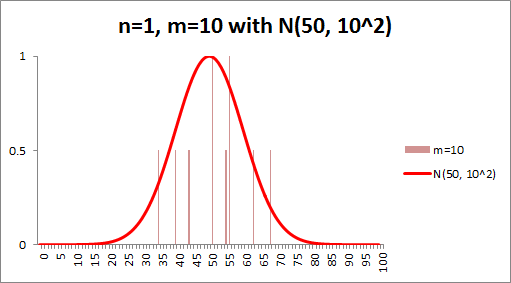
\includegraphics[width=6cm]{./figs/n1m10.png}
	\caption{$n=1, m=10$ のヒストグラムと $N(50, 10^2)$ }
	\label{fig: m10}
\end{minipage}
\begin{minipage}{0.5\hsize}
 \centering
	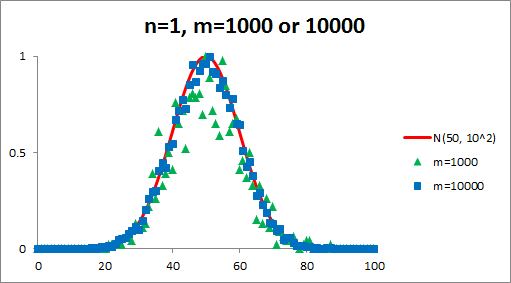
\includegraphics[width=6cm]{./figs/n1m1000_10000.png}
	\caption{$n=1, m=1000 \sim 10000$ の度数分布 }
	\label{fig: m10000}
\end{minipage}
\end{figure}

\subsection{標本の算術平均}

次に、標本の大きさ $n$ を大きくした場合を考えます。
一般に実験で言うところの $n$ 数を多くするわけです。
ただ、$n$ を大きくするだけであれば、繰り返し数の増加と変わらないことになるので、標本の算術平均を取ります。
\begin{align*}
\bar{X} = \dfrac{1}{n} \sum_{i=1}^n x_i
\end{align*}

図 \ref{fig: n3} と \ref{fig: n10} を比較すると、明らかに、$n=10$ の方が母平均 $\mu$ の近傍に集中している、すなわち、分散が小さくなっていることが確認できます。
\begin{figure}[htb]
\begin{minipage}{0.5\hsize}
 \centering
	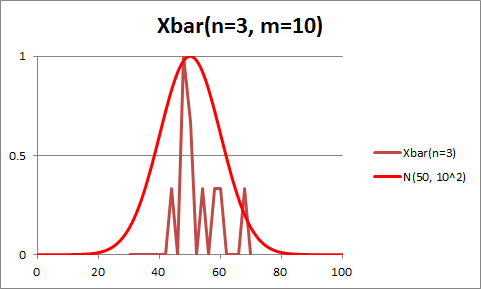
\includegraphics[width=6cm]{./figs/Xbar_n3M10.png}
	\caption{$n=3$ の平均値 $\bar{X} (m=10) $ のヒストグラムと $N(50, 10^2)$ }
	\label{fig: n3}
\end{minipage}
\begin{minipage}{0.5\hsize}
 \centering
	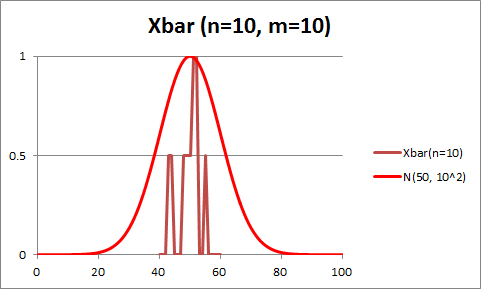
\includegraphics[width=6cm]{./figs/Xbar_n10M10.png}
	\caption{$n=10$ の平均値 $\bar{X} (m=10) $ のヒストグラムと $N(50, 10^2)$ }
	\label{fig: n10}
\end{minipage}
\end{figure}

この結果からだけでは、あまり自明ではないが、$n=3$ でも若干、$n=10$ とした場合にはほぼ明らかに、母集団の正規分布よりも分散が小さくなっているように見える。

このことを確認してみよう。

標本平均 $\bar{X}$ のサンプリング数 $m$ に応じた分散 $V(\bar{X})$ 以下のように算出し、サンプリング数 $m$ でプロットして図に示した。
\begin{align*}
V(\bar{X}) = \dfrac{1}{m} \sum_{j=1}^m [\bar{X}_j - E(\bar{X})]^2
\end{align*}

\begin{figure}[htb]
\begin{minipage}{0.5\hsize}
 \centering
	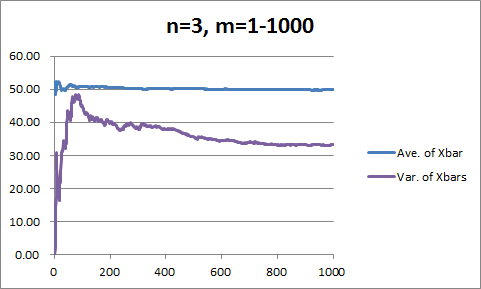
\includegraphics[width=6cm]{./figs/Xbar_n3_m1to1000.png}
	\caption{$n=3$ の平均値 $\bar{X}$ とその分散(サンプリング数:1 to 1000) }
	\label{fig: Xbar_V_n3}
\end{minipage}
\begin{minipage}{0.5\hsize}
 \centering
	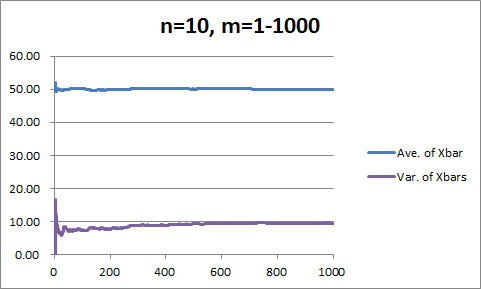
\includegraphics[width=6cm]{./figs/Xbar_n10_m1to1000.png}
	\caption{$n=10$ の平均値 $\bar{X}$ とその分散(サンプリング数:1 to 1000) }
	\label{fig: Xbar_V_n10}
\end{minipage}
\end{figure}
標本平均 $\bar{X}$ のサンプリング数に応じた平均値も併せて図示しています。
どちらの場合においても、標本平均 $\bar{X}$ の平均は素早く母平均 $\mu = 50$ に収束している。

一方、標本平均の分散 $V(\bar{X})$ は $n=3$ では $m$ の増加に伴い、しだいに 33 程度の値に漸近していました。
一方、$n=10$ は、数 100 回程度の繰り返し数で 10 近傍にほぼ収束することが確認できました。

したがって、標本の大きさ $n$ を大きくすることでバラツキを小さく、すなわち、高い確度で母平均を推定できることになります。
しかし、サンプリング数 $m$ の増加に伴い小さな分散へと収束するわけですから、途中の過程ではある程度の変動を伴っていることに注意してください。


\subsection{標本の算術平均の期待値}
\label{sec:V_ave}

ここで、上記の結果について、確率論として確認しましょう。

期待値および分散がそれぞれ $\mu, \sigma^2$ となる確率分布に従う母集団から、大きさ $n$ の標本を取り出して、新たな確率変数 $Y$ を算術平均として以下のように定義します。
\begin{equation*}
Y= \dfrac{X^{(1)} + X^{(2)} + \cdots + X^{(N)} }{N}
\end{equation*}

このとき、$Y$ の期待値は、
\begin{align*}
E(Y)
	&= \bar{X}
\end{align*}

いっぽう、$Y$ の分散 $V(Y)$ は、
\begin{align*}
V(Y)
	&= \dfrac{1}{N} \sigma^2
\end{align*}
となるのであった。

今回は、母集団の分散は $10^2=100$ であったので、$n=3$ の場合は $\dfrac{100}{3} \simeq 33.3$ に、$n=10$ の場合は $\dfrac{100}{10} = 10$ に漸近するものと考えられます。

なお、今回のシミュレーションは推計を行っているのであるから、\ref{sec: EV_sample} に示したように、$m$ の増加に伴いその値に漸近していくことに注意されたい。

\newpage

\section{不偏分散}

\subsection{標本分散と不偏分散}

最後に、標本分散から母分散を推定することを考えよう。

標本の大きさが $n$ であった時、その平均 $\bar{x}$ を用いて、標本分散 $s^2$ は以下のように定義されている。
\begin{align*}
s^2
	&=\dfrac{1}{n} \sum_{i=1}^n (x_i-\bar{x})^2
\end{align*}

教科書では、この標本分散の値は、母分散より小さくなってしまうので、以下の不偏分散 $U$ を使う必要があると書いてある。
\begin{align*}
U
	&=\dfrac{1}{n-1} \sum_{i=1}^n (x_i-\bar{x})^2
\end{align*}

\subsection{シミュレーション}

前述の平均の時と同様な条件で、$n=3, n=10$ の大きさの標本をシミュレートした場合の、それぞれの標本の標本分散 $s^2$ および不偏分散 $U$ を上記の式にしたがって算出し、サンプリング数に応じた平均値としてプロットしました。

母分散は 100 であるが、標本の大きさ $n=3$ では、標本分散は 60 強の値に漸近しており、$n=10$ では 90 程度に収束している。

一方、不偏分散は、どちらの場合も母分散の値である 100 近傍になっている。
\begin{figure}[htb]
\begin{minipage}{0.5\hsize}
 \centering
	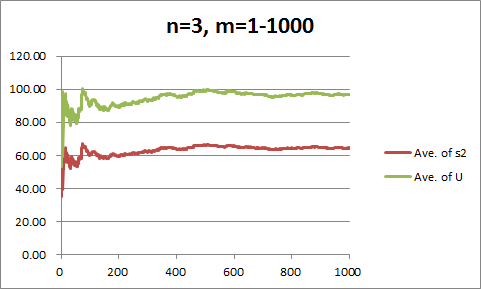
\includegraphics[width=6cm]{./figs/s2_U_n3_m1to1000.png}
	\caption{$n=3$ の標本分散 $s^2$ と 不偏分散 $U$ (サンプリング数:1 to 1000) }
	\label{fig: s2_U_n3}
\end{minipage}
\begin{minipage}{0.5\hsize}
 \centering
	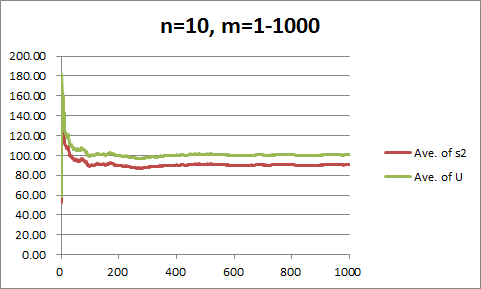
\includegraphics[width=6cm]{./figs/s2_U_n10_m1to1000.png}
	\caption{$n=10$ の平均値 $\bar{X}$ とその分散(サンプリング数:1 to 1000) }
	\label{fig: Xbar_V_n10_2}
\end{minipage}
\end{figure}

\subsection{不偏分散で $n-1$ で割る理由}


上記の標本分散の表式中に、母平均 $\mu$ を導入して展開しよう。
\begin{align*}
s^2
	&=\dfrac{1}{n} \Big[(x_1-\bar{x})^2 + (x_2-\bar{x})^2 + \cdots + (x_n-\bar{x})^2 \Big] \\[6pt]
	&=\dfrac{1}{n} \Big[ \big\{ (x_1-\mu) -(\bar{x} -\mu) \big\}^2 + \big\{ (x_2-\mu) -(\bar{x} -\mu) \big\}^2 + \cdots \\
	&\quad\quad+ \big\{ (x_n-\mu) -(\bar{x} -\mu) \big\}^2 \Big] \\[6pt]
	&=\dfrac{1}{n} \Big[ \big\{ (x_1-\mu)^2 -2(x_1-\mu)(\bar{x} -\mu) +(\bar{x} -\mu)^2 \big\} + \cdots \\
	&\quad\quad + \big\{ (x_n-\mu)^2 -2(x_n-\mu)(\bar{x} -\mu) +(\bar{x} -\mu)^2 \big\} \Big] \\[6pt]
	&=\dfrac{1}{n} \sum_{i=1}^n (x_i-\mu)^2 -2\dfrac{1}{n} \sum_{j=1}^n(x_j-\mu)(\bar{x} -\mu) +\dfrac{1}{n} n (\bar{x} -\mu)^2
\end{align*}
ここで、第二項は以下のように展開できる。
\begin{align*}
 -2\dfrac{1}{n} \sum_{j=1}^n(x_j-\mu)(\bar{x} -\mu) 
	&=  -2(\bar{x} -\mu)\dfrac{1}{n} \sum_{j=1}^n(x_j-\mu) \\[6pt]
	&=  -2(\bar{x} -\mu)(\bar{x} -\mu) \\[6pt]
	&=  -2(\bar{x} -\mu)^2
\end{align*}

この結果を元の式に代入して、
\begin{align*}
s^2
	&=\dfrac{1}{n} \sum_{i=1}^n (x_i-\mu)^2 -2(\bar{x} -\mu)^2 + (\bar{x} -\mu)^2 \\[6pt]
	&=\dfrac{1}{n} \sum_{i=1}^n (x_i-\mu)^2 -(\bar{x} -\mu)^2
\end{align*}

この標本分散の期待値は、
\begin{align*}
E(s^2)
	&=\dfrac{1}{n} \sum_{i=1}^n E [(x_i-\mu)^2] - E[(\bar{x} -\mu)^2]
\end{align*}

この第一項の総和される因子である期待値 $E [(x_i-\mu)^2]$ は、母分散にほかなりません。
また、第二項は、標本平均の母平均まわりでの分散を表しているのだから、前述(\ref{sec:V_ave})の $n$ 個の期待値の算術平均の分散となっている。
したがって、以下のように展開できます。
\begin{align*}
E(s^2)
	&=\dfrac{1}{n} \sum_{i=1}^n E [(x_i-\mu)^2] - E[(\bar{x} -\mu)^2] \\[6pt]
	&=\dfrac{1}{n} (\underbrace{\sigma^2 + \sigma^2 + \cdots + \sigma^2}_{n \text{個}}) - \dfrac{1}{n} \sigma^2 \\[6pt]
	&=\sigma^2 - \dfrac{1}{n} \sigma^2 \\[6pt]
	&=\dfrac{n-1}{n} \sigma^2
% \\[6pt]
%\therefore \quad \sigma^2 &= \dfrac{n}{n-1} E(s^2) = E(U)
\end{align*}

上式より、標本平均の期待値は母分散より $\dfrac{n-1}{n}$ の因子の分だけ小さくなっていることが判る。
したがって、標本平均に $\dfrac{n}{n-1}$ を掛けた $U$ が不偏推定量ということになる。

上述のシミュレーションにおいては、$n=3$ では $\dfrac{3-1}{3}=\dfrac{2}{3}$ だけ、$n=10$ では $\dfrac{10-1}{10}=\dfrac{9}{10}$ だけ母分散より小さくなっている。


\end{document}